% Graphical abstract for EAAI (hand-drawn TikZ, not generative AI).
% Target readable at about 5 x 13 cm; export PDF and upload separately.
\documentclass[12pt]{article}
\usepackage[margin=4mm,paperwidth=13.2cm,paperheight=5.2cm]{geometry}
\usepackage{amsmath}
\usepackage{tikz}
\pagestyle{empty}
\usetikzlibrary{arrows.meta,positioning,calc}
\begin{document}
\noindent\resizebox{\textwidth}{!}{%
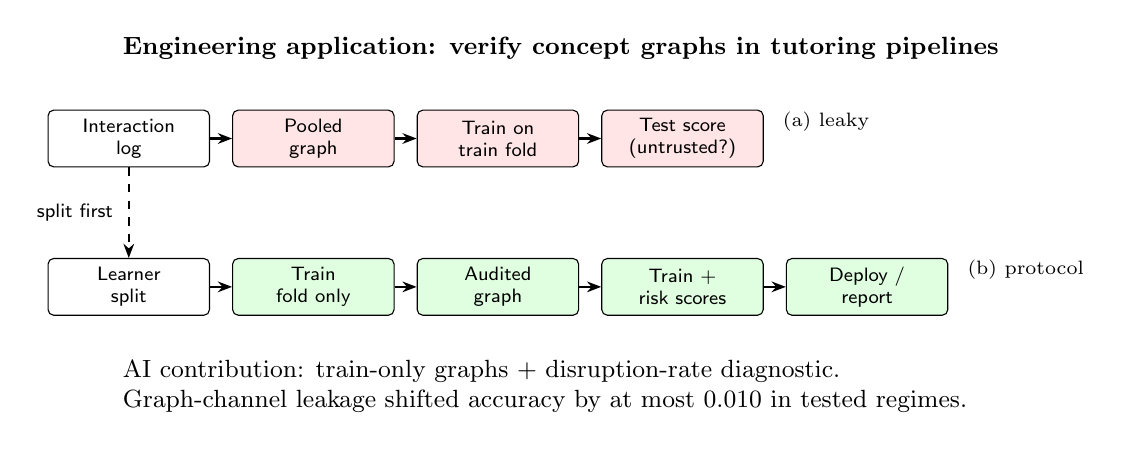
\begin{tikzpicture}[
  font=\sffamily\scriptsize,
  box/.style={draw, rounded corners=2pt, minimum width=2.05cm,
              minimum height=0.72cm, align=center, inner sep=2pt},
  bad/.style={box, fill=red!10},
  good/.style={box, fill=green!12},
  arr/.style={-{Stealth[length=1.8mm]}, thick}
]
\node[font=\small\bfseries, anchor=west] at (-0.2,1.15)
  {Engineering application: verify concept graphs in tutoring pipelines};
\node[box] (log) at (0,0) {Interaction\\log};
\node[bad, right=0.28cm of log] (gfull) {Pooled\\graph};
\node[bad, right=0.28cm of gfull] (m1) {Train on\\train fold};
\node[bad, right=0.28cm of m1] (t1) {Test score\\(untrusted?)};
\draw[arr] (log) -- (gfull);
\draw[arr] (gfull) -- (m1);
\draw[arr] (m1) -- (t1);
\node[font=\scriptsize, anchor=west] at ($(t1.east)+(0.12,0.22)$) {(a) leaky};

\node[box, below=1.15cm of log] (split) {Learner\\split};
\node[good, right=0.28cm of split] (tr) {Train\\fold only};
\node[good, right=0.28cm of tr] (gtrain) {Audited\\graph};
\node[good, right=0.28cm of gtrain] (m2) {Train +\\risk scores};
\node[good, right=0.28cm of m2] (t2) {Deploy /\\report};
\draw[arr] (split) -- (tr);
\draw[arr] (tr) -- (gtrain);
\draw[arr] (gtrain) -- (m2);
\draw[arr] (m2) -- (t2);
\node[font=\scriptsize, anchor=west] at ($(t2.east)+(0.12,0.22)$) {(b) protocol};

\draw[arr, dashed] (log.south) -- (split.north)
  node[midway, left=2pt] {split first};

\node[font=\small, anchor=west, align=left] at (-0.2,-3.15)
  {AI contribution: train-only graphs + disruption-rate diagnostic.\\
   Graph-channel leakage shifted accuracy by at most 0.010 in tested regimes.};
\end{tikzpicture}%
}
\end{document}
